\documentclass[a4paper]{article}
\usepackage[margin=0mm]{geometry}
\usepackage{pdfpages}
\usepackage[hidelinks]{hyperref}

\title{Notebook 2012 -- Samengevoegde LaTeX-uitwerking}
\author{}
\date{}

\begin{document}
\maketitle
\thispagestyle{empty}

\begin{center}
Deze master bundelt alle tot nu toe uitgewerkte paginagroepen.
De originele scan met alle 75 pagina's staat afzonderlijk in dezelfde map.
\end{center}

\clearpage
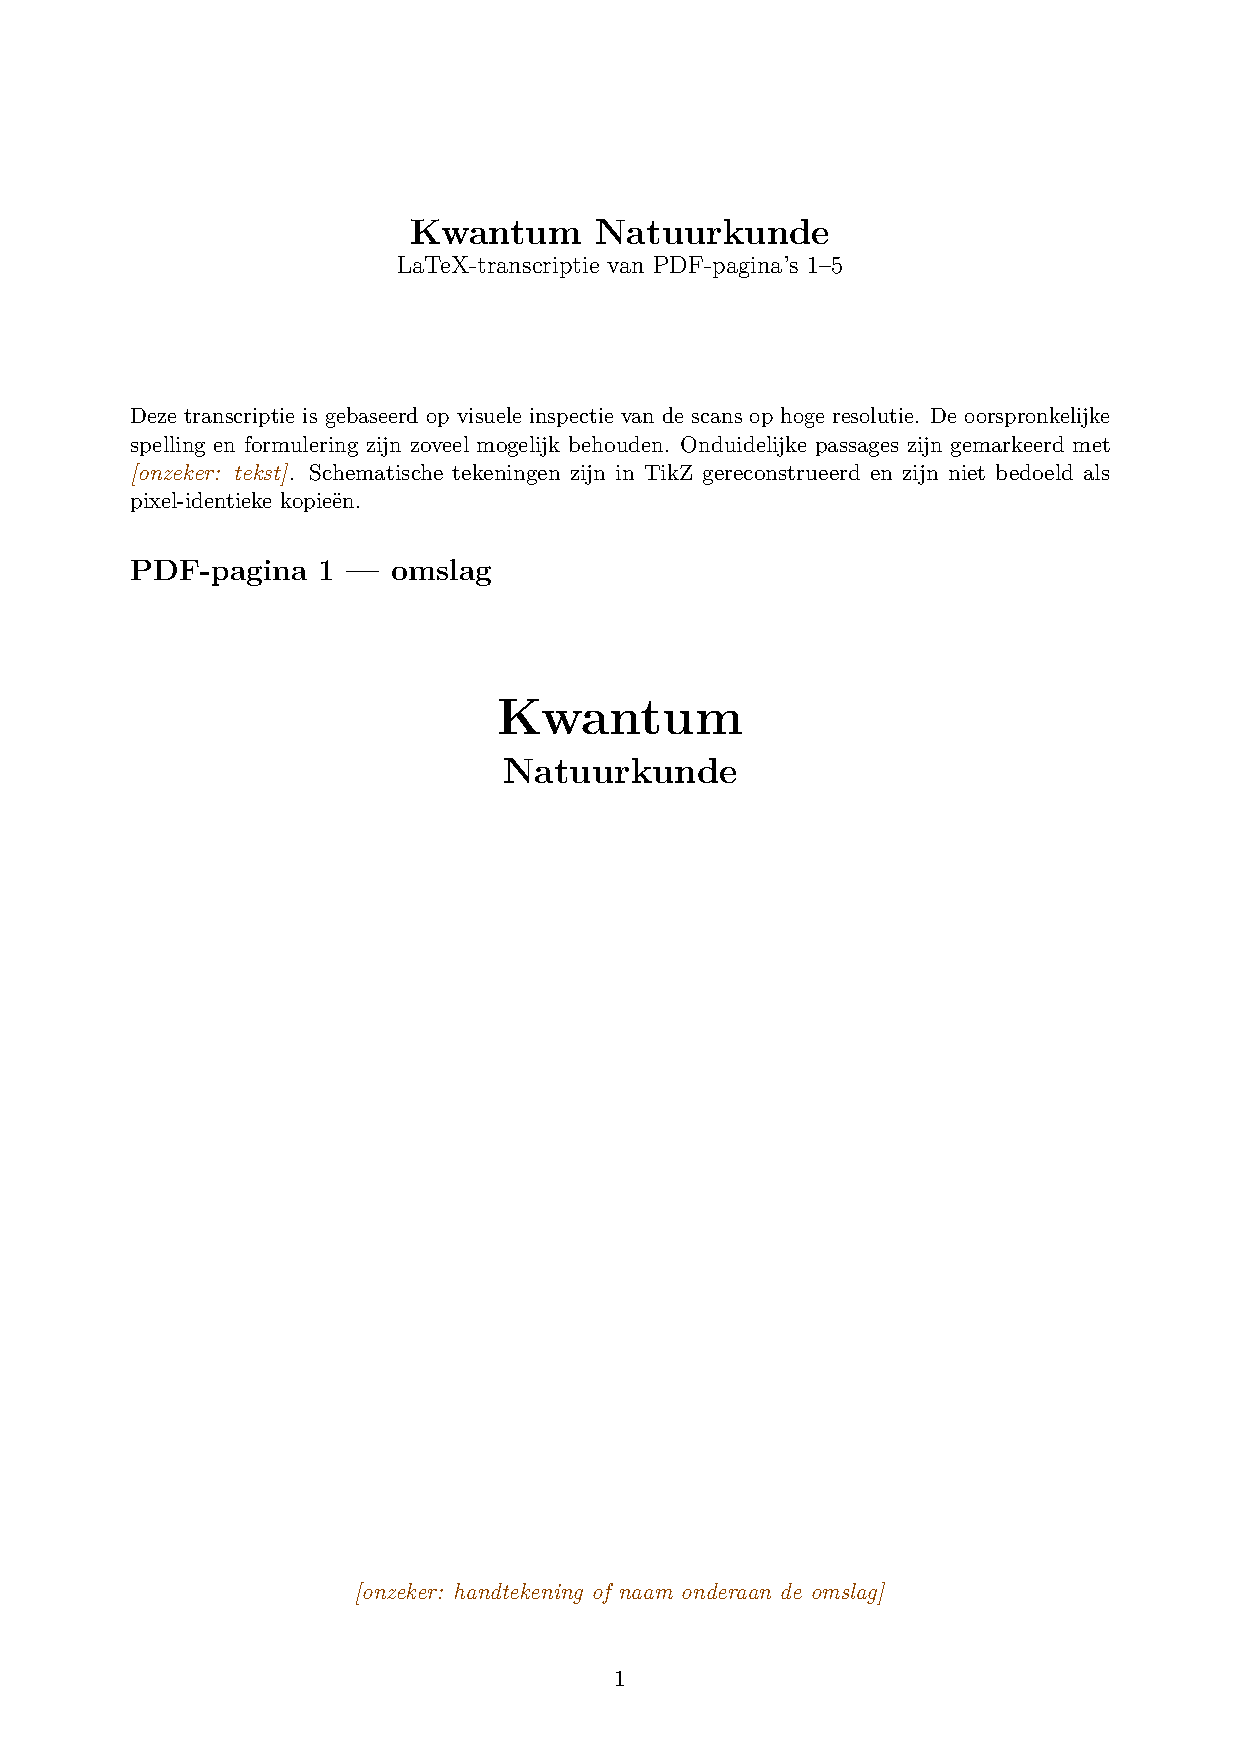
\includepdf[pages=-,pagecommand={\thispagestyle{plain}}]{pdfs/Notebook-2012-paginas-1-5.pdf}

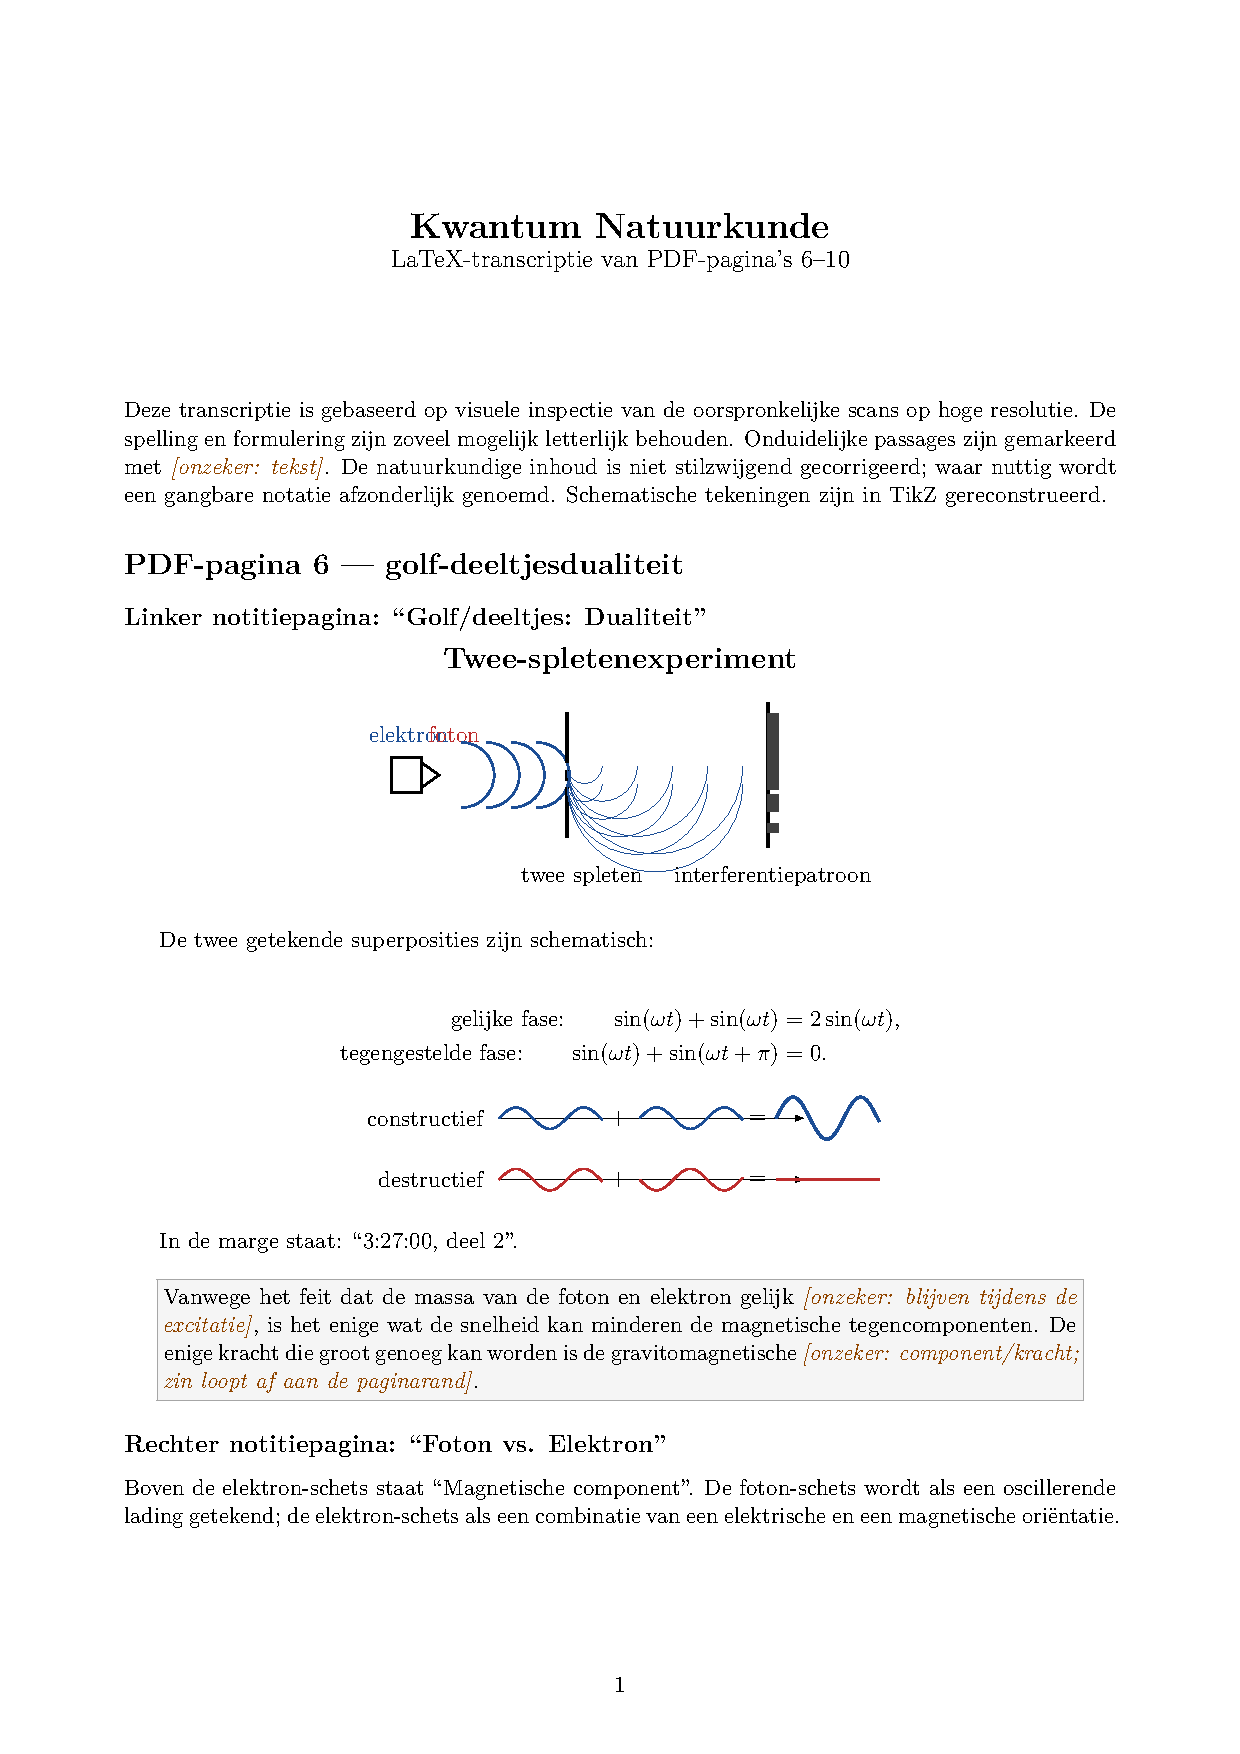
\includepdf[pages=-,pagecommand={\thispagestyle{plain}}]{pdfs/Notebook-2012-paginas-6-10.pdf}

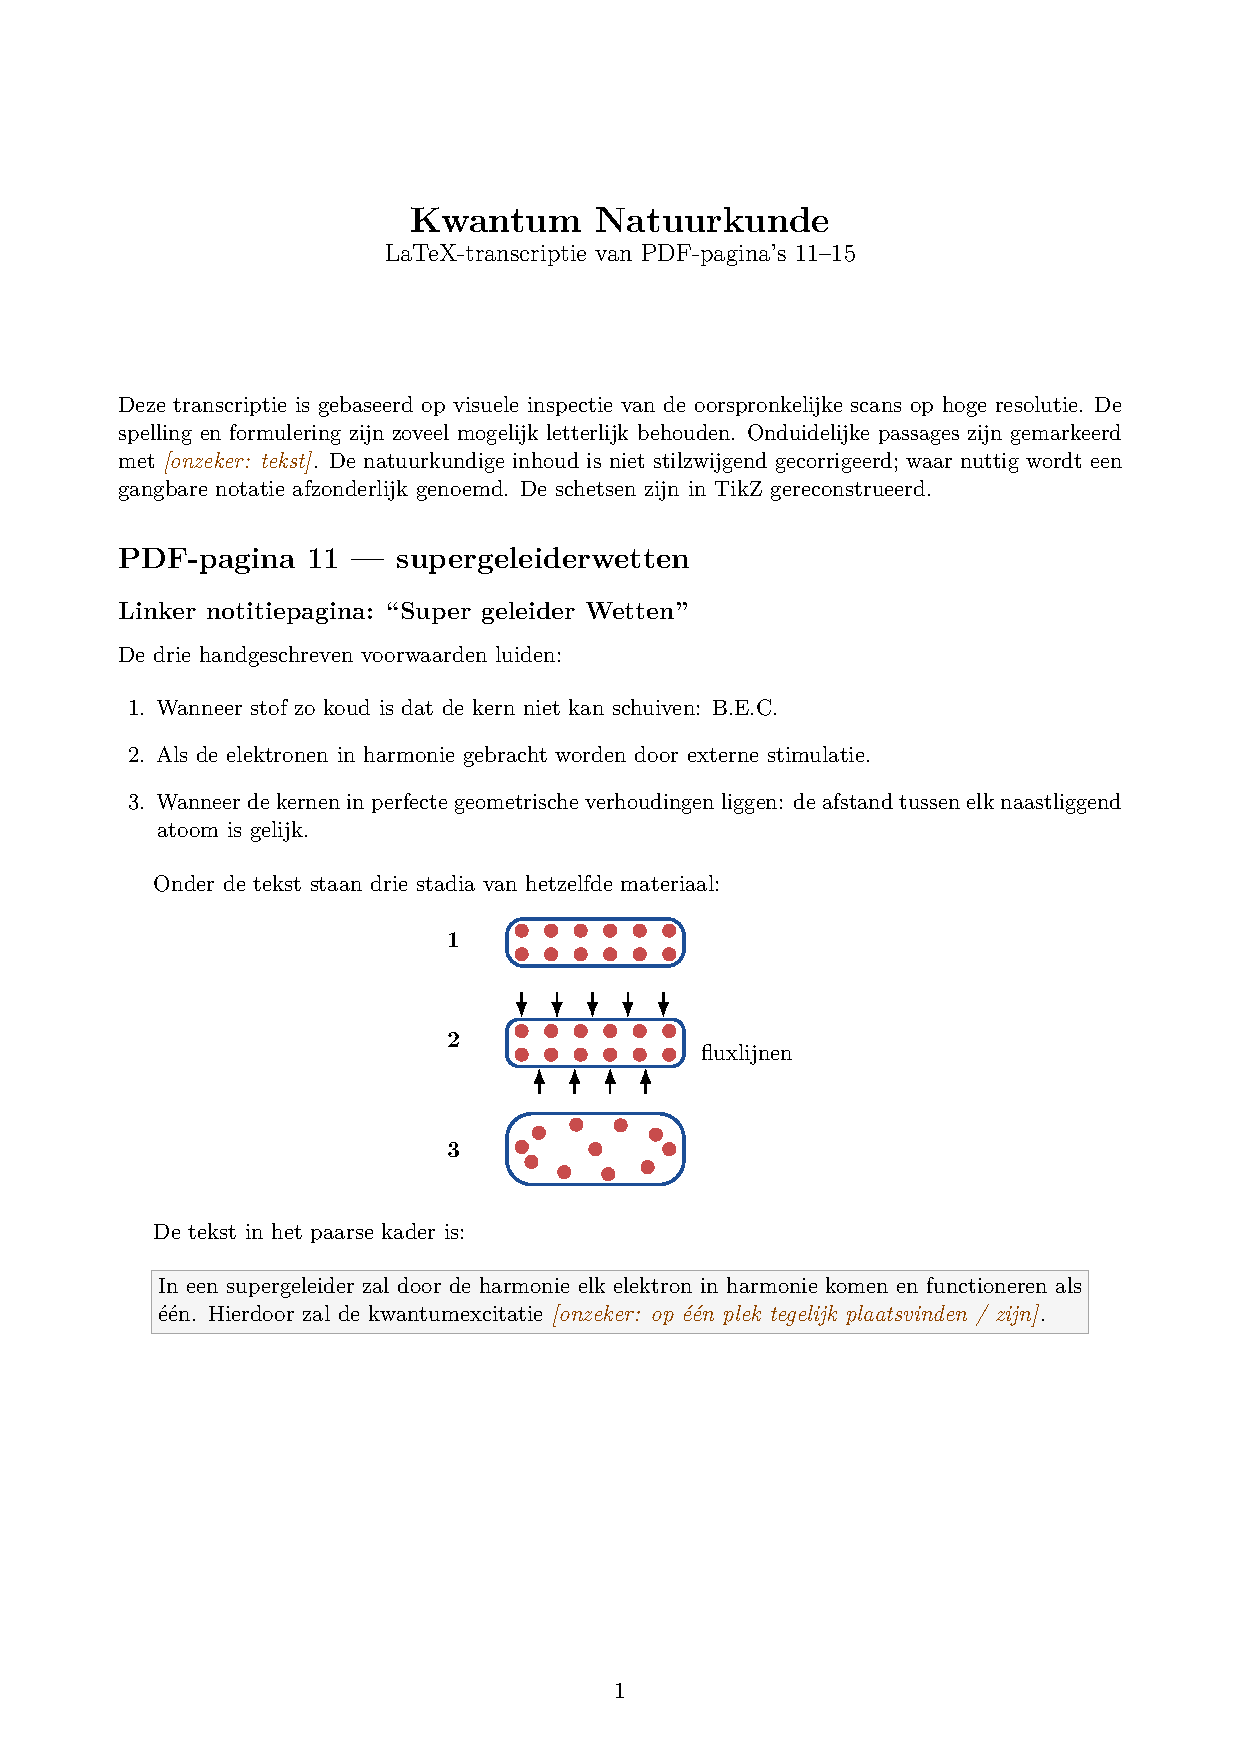
\includepdf[pages=-,pagecommand={\thispagestyle{plain}}]{pdfs/Notebook-2012-paginas-11-15.pdf}

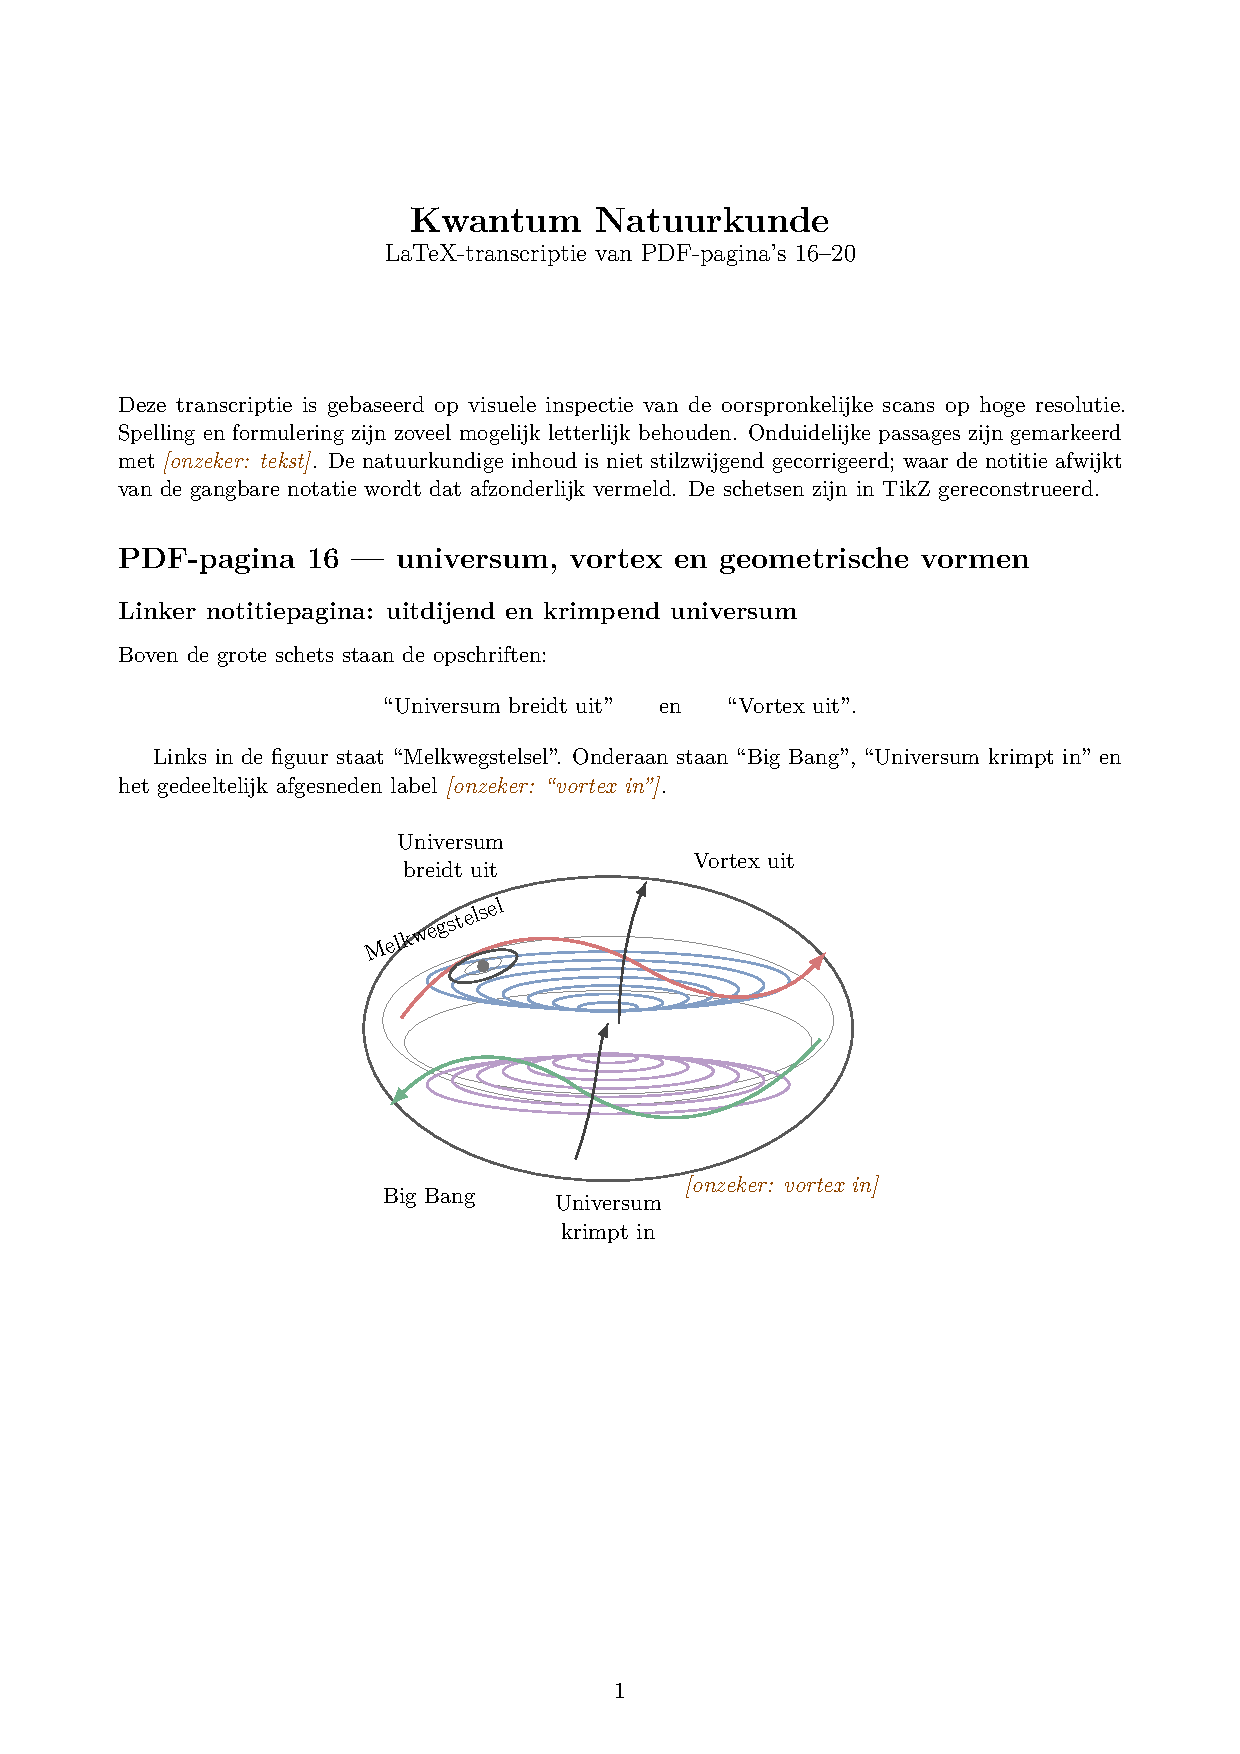
\includepdf[pages=-,pagecommand={\thispagestyle{plain}}]{pdfs/Notebook-2012-paginas-16-20.pdf}

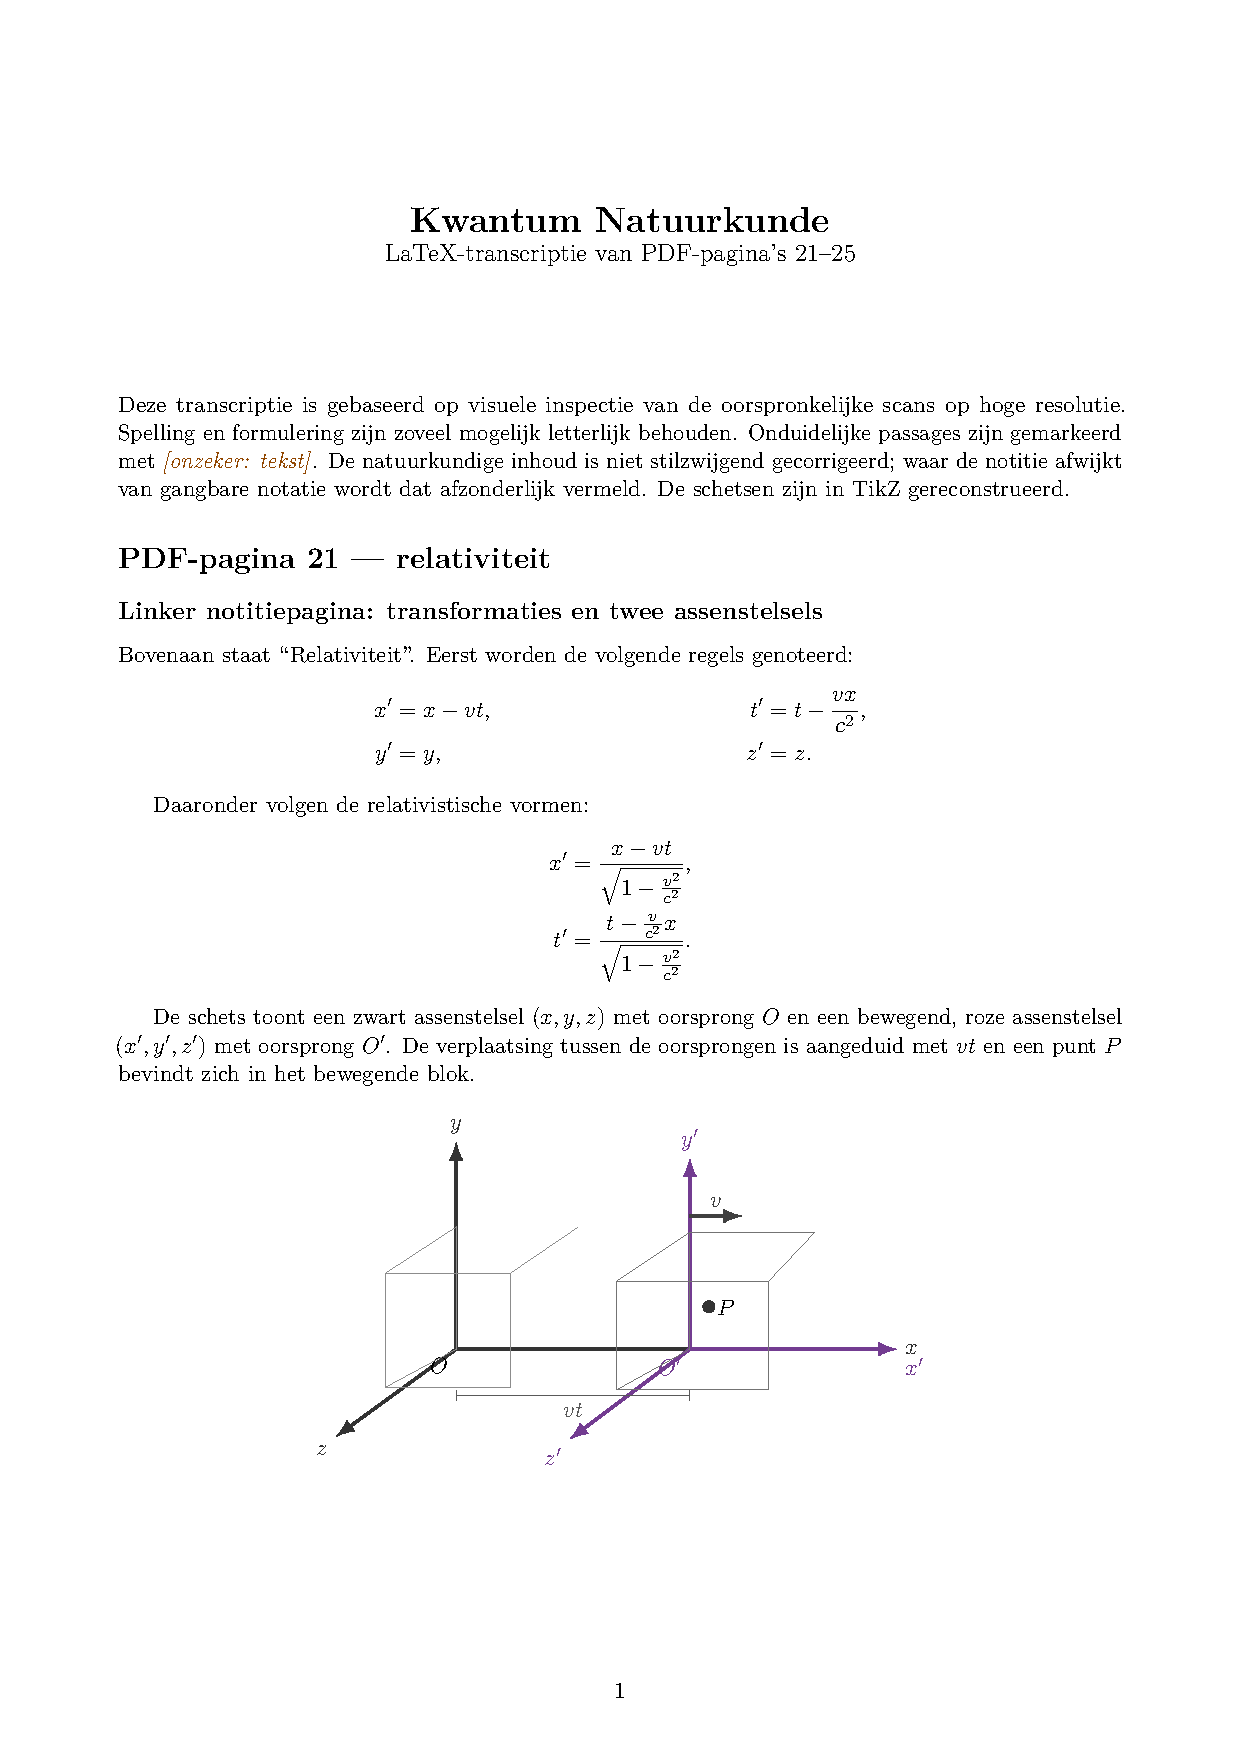
\includepdf[pages=-,pagecommand={\thispagestyle{plain}}]{pdfs/Notebook-2012-paginas-21-25.pdf}


\includepdf[pages=-,pagecommand={\thispagestyle{plain}}]{pdfs/Notebook-2012-paginas-27-31.pdf}


\includepdf[pages=-,pagecommand={\thispagestyle{plain}}]{pdfs/Notebook-2012-paginas-32-36.pdf}


\includepdf[pages=-,pagecommand={\thispagestyle{plain}}]{pdfs/Notebook-2012-paginas-43-47.pdf}


\includepdf[pages=-,pagecommand={\thispagestyle{plain}}]{pdfs/Notebook-2012-paginas-48-50.pdf}


\includepdf[pages=-,pagecommand={\thispagestyle{plain}}]{pdfs/Notebook-2012-paginas-52-54-55.pdf}


\includepdf[pages=-,pagecommand={\thispagestyle{plain}}]{pdfs/Notebook-2012-paginas-65-66-69-72.pdf}

\end{document}
